\documentclass[11pt]{scrartcl}
\usepackage[utf8]{inputenc}
\usepackage{amssymb}
\usepackage[fleqn]{amsmath}
\usepackage{fullpage}
\usepackage{enumitem}
\usepackage{hyperref}
\usepackage{graphicx}
\usepackage{subcaption}
\captionsetup{compatibility=false}
\newcommand{\cX}{\mathcal{X}}
\newcommand{\cR}{\mathcal{R}}
\newcommand{\cV}{\mathcal{V}}
\newcommand{\bw}{\mathbf{w}}
\newcommand{\bb}{\mathbf{b}}

\title{Homework 1}
\author{2020 Spring CSCI 5525: Machine Learning}
\date{Due on Fabruary 16th 11:59pm}


\begin{document}
	\maketitle
	
	Please type in your info:
	\begin{itemize}
		\item \textbf{Name}: Pranay Patil
		\item \textbf{Student ID}: 5592264
		\item \textbf{Email}: patil122@umn.edu
		\item \textbf{Collaborators, and on which problems:}
	\end{itemize}
	
	
	
	
	
	\paragraph{Homework Policy.}
	(1) You are encouraged to collaborate with your classmates on homework problems, but each person must write up the final solutions individually. You need to fill in above to specify which problems were a collaborative effort and with whom. 
	(2) Regarding online resources, you should \textbf{not}:
	\begin{itemize}
		\item  Google around for solutions to homework problems, 
		\item Ask for help on online.
		\item Look up things/post on sites like Quora, StackExchange, etc.
	\end{itemize}
	
	
	%%%%%%%%%%%%%%%%%%%%%%%% SUBMISSION %%%%%%%%%%%%%%%%%%%%%%%%%%%%%%%
	\paragraph{Submission.}
	Submit a PDF using this LaTeX template for written assignment part
	and submit Python jupyter or Colab python notebooks (.ipynb) for all programming part. You should upload all the files on Canvas.
	
	
	
	
	
	\section*{Written Assignment}
	
	\paragraph{Instruction.}
	For each problem, you are required to write down a full mathematical proof to establish the claim. 
	
	\subsection*{Problem 1. Two helpful matrices.}
	Let us first recall the notations in linear regression. The design matrix and the response vector are are defined as:
	\[
	A = \begin{bmatrix} \leftarrow x_1^\intercal \rightarrow \\ \vdots  \\ \leftarrow x_n^\intercal \rightarrow \end{bmatrix} \qquad
	\bb = \begin{pmatrix} y_1 \\ \vdots \\ y_n \end{pmatrix}
	\]
	For this problem, we will assume the covariance matrix $A^\intercal A$ is invertible, and so $(A^\intercal A)^{-1}$ is well-defined (\textbf{Clearly mention the properties of matrix operations used while solving}).
	
	\paragraph{Problem 1.1. The residual matrix.} For any weight vector $\bw$, let us define the vector of least squares residuals as
	\[
	e = \bb  - A \bw
	\]
	Now if $\bw$ is the least square solution given by $\bw = (A^\intercal A)^{-1} A^\intercal \bb$, we can rewrite $e$ as
	\[
	e = \bb - A (A^\intercal A)^{-1} A^\intercal \bb = \left(I - A (A^\intercal A)^{-1} A^\intercal\right)\bb
	\]
	Now let $M = \left(I - A (A^\intercal A)^{-1} A^\intercal\right)$. Show that
	\begin{itemize}
		\item $M$ is symmetric (i.e. $M = M^\intercal$). (\textbf{2 points})
		\item $M$ is idempotent (i.e. $M^2 = M$). (\textbf{2 points})
		\item $M A = 0$. (\textbf{1 point})
	\end{itemize}
	
	%%%%%%%%%%%%%% TYPE YOUR SOLUTION BELOW %%%%%%%%%%%%%%%%%%%%
	\paragraph{Your answer.}
	
	\begin{itemize}
		\item $M$ is symmetric
		
		\textbf{Proof:}
		
		$M = I - A (A^\intercal A)^{-1} A^\intercal$
		
		$M^\intercal = \left(I - A (A^\intercal A)^{-1} A^\intercal\right)^\intercal$
		
		$M^\intercal = I^\intercal - \left(A (A^\intercal A)^{-1} A^\intercal\right)^\intercal$
		
		$M^\intercal = I - \left(A (A^\intercal A)^{-1} A^\intercal\right)^\intercal$
		
		Using $(XZY)^\intercal=Y^\intercal Z^\intercal X^\intercal$
		
		$M^\intercal = I - A \left((A^\intercal A)^{-1}\right)^\intercal A^\intercal$
		
		Using $(X^{-1})^\intercal = (X^\intercal)^{-1}$
		
		$M^\intercal = I - A \left((A^\intercal A)^\intercal\right)^{-1} A^\intercal$
		
		$M^\intercal = I - A (A^\intercal A)^{-1} A^\intercal$
		
		$M^\intercal = M$
		
		\item $M$ is idempotent
		
		\textbf{Proof:}
		
		$M = I - A (A^\intercal A)^{-1} A^\intercal$
		
		$M^2 = \left(I - A (A^\intercal A)^{-1} A^\intercal\right)^2$
		
		Let $H = A (A^\intercal A)^{-1} A^\intercal$
		
		$M^2 = \left(I - H\right)^2$
		
		$M^2 = \left(I - H\right) * \left(I - H\right)$
		
		$M^2 = I\left(I - H\right) - H\left(I - H\right)$
		
		$M^2 = I^2 - IH - HI + H^2$
		
		$M^2 = I^2 - 2H + H^2$
		
		Now, 
		
		$H^2 = \left(A (A^\intercal A)^{-1} A^\intercal\right)^2$
		
		$H^2 = \left(A (A^\intercal A)^{-1} A^\intercal\right) * \left(A (A^\intercal A)^{-1} A^\intercal\right)$
		
		$H^2 = A [(A^\intercal A)^{-1} (A^\intercal A)] (A^\intercal A)^{-1} A^\intercal $
		
		$H^2 = A I (A^\intercal A)^{-1} A^\intercal $
		
		$H^2 = A (A^\intercal A)^{-1} A^\intercal $
		
		$H^2 = H$
		
		Therefore,
		
		$M^2 = I^2 - 2H + H$
		
		$M^2 = I^2 - H$
		
		$M^2 = I - A (A^\intercal A)^{-1} A^\intercal$
		
		$M^2 = M$
		
		\item $MA = 0$
		
		\textbf{Proof:}
		
		$MA = \left(I - A (A^\intercal A)^{-1} A^\intercal\right) A$
		
		$MA = A - A (A^\intercal A)^{-1} (A^\intercal A)$
		
		$MA = A - AI$
		
		$MA = A - A$
		
		$MA = 0$
	\end{itemize}
	
	
	
	%%%%%%%%%%%%%% TYPE YOUR SOLUTION ABOVE %%%%%%%%%%%%%%%%%%%%
	
	
	\paragraph{Problem 1.2. The hat matrix.} Using the residual maker, we can derive another matrix, the hat matrix or projection matrix $P = I - M =  A (A^\intercal A)^{-1} A^\intercal$. Note that the predicted value by the least squares solution is given by $P \bb$.
	Show that 
	\begin{itemize}
		\item $P$ is symmetric. (\textbf{1 point})
		\item $P$ is idempotent. (\textbf{1 point})
	\end{itemize}
	
	%%%%%%%%%%%%%% TYPE YOUR SOLUTION BELOW %%%%%%%%%%%%%%%%%%%%
	\paragraph{Your answer.}
	
	\begin{itemize}
		\item $P$ is symmetric
		
		\textbf{Proof:}
		
		$P = A (A^\intercal A)^{-1} A^\intercal$\\
		$P^\intercal = \left(A (A^\intercal A)^{-1} A^\intercal\right)^\intercal$\\
		$P^\intercal = A \left((A^\intercal A)^{-1}\right)^\intercal A^\intercal$\\
		$P^\intercal = A \left((A^\intercal A)^\intercal\right)^{-1} A^\intercal$\\
		$P^\intercal = A (A^\intercal A)^{-1} A^\intercal$\\
		$P^\intercal = P$\\
		
		\item $P$ is idempotent
		
		\textbf{Proof:}
		
		$P = A (A^\intercal A)^{-1} A^\intercal$\\
		$P^2 = \left(A (A^\intercal A)^{-1} A^\intercal\right)^2$\\
		$P^2 = \left(A (A^\intercal A)^{-1} A^\intercal\right) * \left(A (A^\intercal A)^{-1} A^\intercal\right)$\\
		$P^2 = A (A^\intercal A)^{-1} (A^\intercal A) (A^\intercal A)^{-1} A^\intercal $\\
		$P^2 = A I (A^\intercal A)^{-1} A^\intercal $\\
		$P^2 = A (A^\intercal A)^{-1} A^\intercal $\\
		$P^2 = P$
	\end{itemize}
	
	
	
	
	%%%%%%%%%%%%%% TYPE YOUR SOLUTION ABOVE %%%%%%%%%%%%%%%%%%%%
	
	
	\subsection*{Problem 2. Gradient of conditional log-likelihood.}
	For any $a\in \mathbb{R}$, let  $\sigma(a) = \frac{1}{1 +\exp(-a)}$.
	For each example $(x_i, y_i)\in \mathbb{R}^d \times \{0, 1\}$, the conditional log-likelihood of logistic regression is
	\[
	\ell(y_i \mid x_i, \bw) = y_i \ln(\sigma(\bw^\intercal x_i)) + (1 - y_i)\ln(\sigma(-\bw^\intercal x_i))
	\]
	Derive the gradient of $\ell(y_i\mid x_i, \bw)$ with respect to $w_j$ (i.e. the $j$-th coordinate of $\bw$), i.e. $\frac{\partial }{\partial w_j}\ell(y_i \mid x_i, \bw)$  (\textbf{Clearly mention the properties of derivatives used while solving}). (\textbf{6 points})
	
	%%%%%%%%%%%%%% TYPE YOUR SOLUTION BELOW %%%%%%%%%%%%%%%%%%%%
	\paragraph{Your answer.}
	First consider the function $\sigma(a)$\\
	\begin{gather*}
	\sigma(a) = \frac{1}{1 +\exp(-a)}\\
	Taking\ derivative\ w.r.t.\ a\\
	\frac{\partial }{\partial a}\sigma(a) = \frac{\partial }{\partial a}[\frac{1}{1 +\exp(-a)}]\\
	By\ chain\ rule\\
	\frac{\partial }{\partial a}\sigma(a) = -1 * \frac{1}{(1+\exp(-a))^{2}} * \frac{\partial }{\partial a}\exp(-a)\\
	\frac{\partial }{\partial a}\sigma(a) = -1 * \frac{1}{(1+\exp(-a))^{2}} * \exp(-a) * -1\\
	\frac{\partial }{\partial a}\sigma(a) = \frac{\exp(-a)}{(1+\exp(-a))^{2}}\\
	\frac{\partial }{\partial a}\sigma(a) = \frac{1+\exp(-a)-1}{(1+\exp(-a))^{2}}\\
	\frac{\partial }{\partial a}\sigma(a) = \frac{1+\exp(-a)}{(1+\exp(-a))^{2}} - \frac{1}{(1+\exp(-a))^{2}}\\
	\frac{\partial }{\partial a}\sigma(a) = \frac{1}{(1+\exp(-a))} - \frac{1}{(1+\exp(-a))^{2})}\\
	\frac{\partial }{\partial a}\sigma(a) = \frac{1}{1+\exp(-a)}[1 - \frac{1}{(1+\exp(-a)}]\\
	\end{gather*}
	\begin{gather}
	\frac{\partial }{\partial a}\sigma(a) = \sigma(a)(1-\sigma(a))
	\end{gather}
	Now consider the conditional log likelihood:
	\begin{gather*}
	l(y_i\mid x_i,w) = y_i \ln(\sigma(w^\intercal x_i)) + (1 - y_i)\ln(\sigma(-w^\intercal x_i))\\
	Taking\ derivative\ w.r.t.\ w_j\\
	\frac{\partial }{\partial w_j}l(y_i\mid x_i,w) = \frac{\partial }{\partial w_j}[y_i \ln(\sigma(w^\intercal x_i)) + (1 - y_i)\ln(\sigma(-w^\intercal x_i))]\\
	Distributing\ differential\\
	\frac{\partial }{\partial w_j}l(y_i\mid x_i,w) = \frac{\partial }{\partial w_j}[y_i \ln(\sigma(w^\intercal x_i))] + \frac{\partial }{\partial w_j}[(1 - y_i)\ln(\sigma(-w^\intercal x_i))]\\
	\frac{\partial }{\partial w_j}l(y_i\mid x_i,w) = y_i*\frac{\partial }{\partial w_j}[ \ln(\sigma(w^\intercal x_i))] + (1 - y_i)*\frac{\partial }{\partial w_j}[\ln(\sigma(-w^\intercal x_i))]\\
	But\ \sigma(-a) = 1-\sigma(a)\\
	\frac{\partial }{\partial w_j}l(y_i\mid x_i,w) = y_i*\frac{\partial }{\partial w_j}[ \ln(\sigma(w^\intercal x_i))] + (1 - y_i)*\frac{\partial }{\partial w_j}[\ln(1 - \sigma(w^\intercal x_i))]\\
	By\ chain\ rule\\
	\frac{\partial }{\partial w_j}l(y_i\mid x_i,w) = y_i*\frac{1}{\sigma(w^\intercal x_i)} \frac{\partial }{\partial w_j}\sigma(w^\intercal x_i) + (1 - y_i)*\frac{1}{1-\sigma(w^\intercal x_i)} \frac{\partial }{\partial w_j}(1-\sigma(w^\intercal x_i))\\
	\frac{\partial }{\partial w_j}l(y_i\mid x_i,w) = y_i*\frac{1}{\sigma(w^\intercal x_i)} \frac{\partial }{\partial w_j}\sigma(w^\intercal x_i) - (1 - y_i)*\frac{1}{1-\sigma(w^\intercal x_i)} \frac{\partial }{\partial w_j}\sigma(w^\intercal x_i)\\
	\frac{\partial }{\partial w_j}l(y_i\mid x_i,w) = \frac{\partial }{\partial w_j}\sigma(w^\intercal x_i)(y_i*\frac{1}{\sigma(w^\intercal x_i)} - (1 - y_i)*\frac{1}{1-\sigma(w^\intercal x_i)})\\
	From\ (1)\ and\ chain\ rule\\
	\frac{\partial }{\partial w_j}l(y_i\mid x_i,w) = \sigma(w^\intercal x_i)(1-\sigma(w^\intercal x_i))\frac{\partial }{\partial w_j}w^\intercal x_i(y_i*\frac{1}{\sigma(w^\intercal x_i)} - (1 - y_i)*\frac{1}{1-\sigma(w^\intercal x_i)})\\
	\frac{\partial }{\partial w_j}l(y_i\mid x_i,w) = \frac{\partial }{\partial w_j}w^\intercal x_i(y_i*\frac{\sigma(w^\intercal x_i)(1-\sigma(w^\intercal x_i))}{\sigma(w^\intercal x_i)} - (1 - y_i)*\frac{\sigma(w^\intercal x_i)(1-\sigma(w^\intercal x_i))}{1-\sigma(w^\intercal x_i)})\\
	\frac{\partial }{\partial w_j}l(y_i\mid x_i,w) = \frac{\partial }{\partial w_j}w^\intercal x_i(y_i(1-\sigma(w^\intercal x_i)) - (1-y_i)\sigma(w^\intercal x_i))\\
	\frac{\partial }{\partial w_j}l(y_i\mid x_i,w) = \frac{\partial }{\partial w_j}w^\intercal x_i(y_i- y_i*\sigma(w^\intercal x_i) - \sigma(w^\intercal x_i)+y_i*\sigma(w^\intercal x_i))\\
	\frac{\partial }{\partial w_j}l(y_i\mid x_i,w) = \frac{\partial }{\partial w_j}w^\intercal x_i(y_i - \sigma(w^\intercal x_i))\\
	Now\ w^\intercal x_i = w_1 x_{i1} + w_2 x_{i2} + . . . + w_n x_{in},\\
	so\ \frac{\partial }{\partial w_j}w^\intercal x_i = 0 + 0 + ...\frac{\partial }{\partial w_j}w_j x_{ij}...+ 0\\
	\frac{\partial }{\partial w_j}l(y_i\mid x_i,w) = x_{ij}(y_i - \sigma(w^\intercal x_i))\\
	\end{gather*}
	
	
	
	
	%%%%%%%%%%%%%% TYPE YOUR SOLUTION ABOVE %%%%%%%%%%%%%%%%%%%%
	
	
	\subsection*{Problem 3. Derivation of Ridge Regression Solution.}
	Recall that in class we claim that the solution to ridge regression ERM:
	\[
	\min_{\bw} \hspace{5pt}(\|A \bw - \bb\|_2^2 + \lambda \|\bw\|_2^2)
	\]
	is $\bw^* = (A^\intercal A + \lambda I)^{-1}A^\intercal \bb$. Now provide a proof. (\textbf{6 points})\\
	(Hint: recall that $\nabla F(\bw) = \textbf{0}$ is a sufficient condition for $\bw$ to be a minimizer of any convex function $F$. To get a full credit, you should be able to show why $A^\intercal A + \lambda I$ is invertible.)
	(\textbf{Clearly mention the properties of matrix calculus used while solving})
	%%%%%%%%%%%%%% TYPE YOUR SOLUTION BELOW %%%%%%%%%%%%%%%%%%%%
	\paragraph{Your answer.}
	\begin{gather*}
	F(w) = \min_w(\|Aw-b\|_2^2 + \lambda\|w\|_2^2)\\
	Differentiating\ F(w)\ wrt\ w\\
	\nabla F(\bw) = \frac{\partial }{\partial w}F(w)\\
	\nabla F(\bw) = \frac{\partial }{\partial w}(\|Aw-b\|_2^2 + \lambda\|w\|_2^2)\\
	\nabla F(\bw) = \frac{\partial }{\partial w}\|Aw-b\|_2^2 + \frac{\partial }{\partial w}\lambda\|w\|_2^2\\
	\nabla F(\bw) = 2(Aw-b) \frac{\partial }{\partial w}Aw + 2\lambda w\\
	\nabla F(\bw) = 2A^\intercal(Aw-b) + 2\lambda w\\
	To\ minimize\ F(w)\ we\ will\ equate\ \nabla F(\bw^*)\ to\ 0\\
	2A^\intercal(Aw^*-b) + 2\lambda w^* = 0\\
	A^\intercal(Aw^*-b) + \lambda w^* = 0\\
	A^\intercal Aw^*- A^\intercal b + \lambda w^* = 0\\
	A^\intercal Aw^* + \lambda w^* = A^\intercal b \\
	w^*(A^\intercal A + \lambda I)= A^\intercal b \\
	w^*= (A^\intercal A + \lambda I)^{-1}A^\intercal b
	\end{gather*}
	Here, since we are adding a positive constant $\lambda$ to the diagonal of $A^\intercal A$, $A^\intercal A + \lambda I$ it will always be invertible, even for the cases where $A^\intercal A$ is singular.\\
	To prove that $w^*$ is the optimal minimizer, we can verify if the $2^{nd}$ derivative of $F(w)$ is positive:
	\begin{gather*}
	From\ above\ calculations\\
	\nabla^2 F(\bw) =  \frac{\partial }{\partial w}(2A^\intercal Aw + 2\lambda w - 2A^\intercal b)\\
	\nabla^2 F(\bw) =  \frac{\partial }{\partial w}2A^\intercal Aw + \frac{\partial }{\partial w}2\lambda w - \frac{\partial }{\partial w}2A^\intercal b\\
	\nabla^2 F(\bw) =  2A^\intercal A + 2\lambda
	\end{gather*}
	It can be seen that $A^\intercal A$ is just a square of values in A and $\lambda$ is a positive constant. Hence $\nabla^2 F(\bw) > 0$ and $w^*$ is an optimal solution for $\min_w(\|Aw-b\|_2^2 + \lambda\|w\|_2^2)$
	
	
	%%%%%%%%%%%%%% TYPE YOUR SOLUTION ABOVE %%%%%%%%%%%%%%%%%%%%
	
	\subsection*{Problem 4. Minimizing a Squared Norm Plus an Affine Function.}
	A generalization of the least squares
	problem adds an affine function to the least squares objective,
	\[
	\min_{\bw} \hspace{5pt} \|A \bw - \bb\|_2^2 + c^\intercal \bw + d
	\]
	where $A \in \mathbb{R}^{m \times n}, \bw\in \mathbb{R}^n, \bb \in \mathbb{R}^m, c \in \mathbb{R}^n, d \in \mathbb{R}$. Assume the column of $A$ are linearly independent.
	This generalized problem can be solved by reducing it to a standard least squares problem, using a trick called \textit{completing the square}.
	
	Show that the objective of the problem above can be expressed in the form
	
	\[
	\|A \bw - \bb\|_2^2 + c^\intercal \bw + d = \|A \bw - \bb + \mathbf{f}\|_2^2 + g
	\]
	where $ \mathbf{f} \in \mathbb{R}^m, g \in \mathbb{R}$.It follows that we can solve the generalized least squares problem by minimizing $\|A \bw - (\bb - \mathbf{f})\|_2^2$
	
	(Hint: Express the norm squared term on the right-hand side as $\| (A \bw - \bb) + \mathbf{f})\|_2^2$ and
	expand it. Then argue that the equality above holds provided $2A^\intercal \textbf{f} = c$. One possible choice is $f = \frac{1}{2}(A^\dagger)^\intercal c$.) (You must justify these statements.) (\textbf{6 point})
	%%%%%%%%%%%%%% TYPE YOUR SOLUTION BELOW %%%%%%%%%%%%%%%%%%%%
	\paragraph{Your answer.}
	
	To prove the first part we will start from the RHS:
	\begin{gather*}
	\|Aw - b + f\|_2^2 + g = \|(Aw - b) +f\|_2^2 + g\\
	\|Aw - b + f\|_2^2 + g = (Aw-b)^\intercal(Aw-b) + 2f^\intercal (Aw-b)+f^\intercal f + g\\
	\|Aw - b + f\|_2^2 + g = \|(Aw - b) +f\|_2^2 + 2f^\intercal Aw - 2f^\intercal b + f^\intercal f + g\\
	\|Aw - b + f\|_2^2 + g = \|(Aw - b) +f\|_2^2 + 2f^\intercal Aw + f^\intercal (f - 2b) + g\\
	\end{gather*}
	Comparing '$\|(Aw - b) +f\|_2^2 + 2f^\intercal Aw + f^\intercal (f - 2b) + g$' to '$\|A - b\|_2^2 + c^\intercal w + d$' we get:
	\begin{gather*}
	c^\intercal w = 2f^\intercal Aw\\
	d = f^\intercal (f - 2b) + g\\
	\end{gather*}
	For the second part:\\
	We know that
	\begin{gather*}
	2f^\intercal Aw = c^\intercal w\\
	2f^\intercal Aw - c^\intercal w = 0\\
	2(A^\intercal f)^\intercal w - c^\intercal w = 0\\
	(2(A^\intercal f)^\intercal - c^\intercal )w = 0
	\end{gather*}
	This holds if $2(A^\intercal f)^\intercal = c^\intercal$ or simply $2A^\intercal f = c$\\
	To justify the possible value of f given in the hint, lets substitute it in the above equation
	
	\begin{flalign*}
	2A^\intercal f = 2A^\intercal \frac{1}{2}(A^\dagger)^\intercal c\\
	Now, A^\dagger = (A^\intercal A)^{-1}A^\intercal\\
	2A^\intercal f = 2A^\intercal \frac{1}{2}((A^\intercal A)^{-1}A^\intercal)^\intercal c\\
	2A^\intercal f = A^\intercal (A((A^\intercal A)^{-1})^\intercal) c\\
	2A^\intercal f = A^\intercal (A((A^\intercal A)^\intercal)^{-1}) c\\
	2A^\intercal f = A^\intercal A((A^\intercal A)^\intercal)^{-1} c\\
	2A^\intercal f = A^\intercal A(A^\intercal A)^{-1} c\\
	2A^\intercal f = (A^\intercal A)(A^\intercal A)^{-1} c\\
	2A^\intercal f = Ic\\
	2A^\intercal f = c\\
	\end{flalign*}
	
	%%%%%%%%%%%%%% TYPE YOUR SOLUTION ABOVE %%%%%%%%%%%%%%%%%%%%
	
	\subsection*{Problem 5. Iterative Method for Least Squares Problem.}
	
	In this exercise we explore an iterative method, due to the mathematician Lewis Richardson, that can be used to compute $\hat{\bw} = A^\dagger \bb$, we define $\bw^{(1)} = 0$ and for $k = 1, 2, 3, ...,$
	$$
	\bw^{(k+1)} = \bw^{(k)} - \mu A^\intercal (A\bw^{(k)} - \bb)
	$$
	where $\mu$ is a positive parameter, and the superscripts denote the iteration number.This defines a sequence of vectors that converge to $\hat{\bw}$ provided $\mu$ is not too large; The iteration is terminated when $A^\intercal (A \bw^{(k)} - \bb)$ is small enough, which means the least squares optimality conditions are almost satisfied. To implement the method we only need to multiply vectors by $A$ and by $A^\intercal$. If we have efficient methods for carrying out these two matrix-vector multiplications, this iterative
	method can be faster. Iterative methods are often used for very large scale least squares problems.
	\begin{itemize}
		\item [(a)] Show that if $\bw ^{(k+1)} = \bw ^{(k)}$, we have $\bw^{(k)} = \hat{\bw}$.  (\textbf{5 points})
		\item [(b)] Express the vector sequence $x^{(k)}$ as a linear dynamical system with constant dynamics matrix and offset, i.e., in the form $\bw^{(k+1)} = F\bw^{(k)} + g$.  (\textbf{3 points})
	\end{itemize}
	
	%%%%%%%%%%%%%% TYPE YOUR SOLUTION BELOW %%%%%%%%%%%%%%%%%%%%
	\paragraph{Your answer (a)}
	Solution to the least square solutions is given by,
	\begin{gather*}
	f(w) = \|Aw - b\|_2^2\\
	Differentiating\ wrt\ to\ w\ get\ the\ optimal\ solution\\
	\nabla f(w) = \frac{\partial }{\partial w}\|Aw - b\|_2^2\\
	\nabla f(w) = 2A^\intercal (Aw-b)\\
	If\ \hat{w}\ is\ the\ optimum\ solution,\ then\ \nabla f(w) = 0\\
	2A^\intercal (A\hat{w}-b) = 0\\
	A^\intercal (A\hat{w}-b) = 0\\
	This\ is\ first\ order\ condition
	\end{gather*}
	
	Now, consider the given iterative solution:
	\begin{gather*}
	w^{(k+1)}=w^{(k)}-\mu A^\intercal(Aw^{(k)}-b)\\
	If\ w^{(k+1)} = w^{(k)},\\
	w^{(k)}=w^{(k)}-\mu A^\intercal(Aw^{(k)}-b)\\
	\mu A^\intercal(Aw^{(k)}-b)=w^{(k)}-w^{(k)}\\
	\mu A^\intercal(Aw^{(k)}-b) = 0\\
	A^\intercal(Aw^{(k)}-b) = 0\\
	From\ first\ order\ condition,\ w^{(k)} is\ the\ optimal\ solution\\
	w^{(k)} = \hat{w}
	\end{gather*}
	\paragraph{Your answer (b)}
	\begin{gather*}
	w^{(k+1)}=w^{(k)}-\mu A^\intercal(Aw^{(k)}-b)\\
	w^{(k+1)}=w^{(k)}-\mu A^\intercal Aw^{(k)} + \mu A^\intercal b\\
	w^{(k+1)}=(I-\mu A^\intercal A)w^{(k)} + (\mu A^\intercal b)\\
	w^{(k+1)}=Fw^{(k)} + g\\
	where,\\
	F = constant\ dynamics\ matrix = I-\mu A^\intercal A\\
	g = offset = \mu A^\intercal b
	\end{gather*}
	
	
	
	
	
	%%%%%%%%%%%%%% TYPE YOUR SOLUTION ABOVE %%%%%%%%%%%%%%%%%%%%
	
	%%%%%%%%%%%%%%%%%%%%%%%%%%%%%%%%%%%%%%%%%%%%%%%%%%%%%%%%%%%%%%%%%%%%%%%%%%%%%%%
	\newpage
	%%%%%%%%%%%%%%%%%%%%%%%% PROGRAMMING ASSIGNMENT %%%%%%%%%%%%%%%%%%%%%%%%%%%%%%%
	\section*{Programming Assignment}
	
	\paragraph{Instruction.}
	For each problem, you are required to report descriptions and results in the PDF and submit code as python file (.py) (as per the question). 
	
	\begin{itemize}
		\item \textbf{Python} version: Python 3.
		\item Please follow PEP 8 style of writing your Python code for better readability in case you are wondering how to name functions \& variables, put comments and indent your code
		
		\item \textbf{Packages allowed}: numpy, pandas, matplotlib
		
		\item Please PROPERLY COMMENT your code in order to have utmost readability 
		
		\item Please provide the required functions for each problem.
		
		\item There shall be NO runtime errors involved.
		
		\item There would be PENALTY if any of the above is not followed
		
		\item \textbf{Submission}: For programming parts, \textbf{ONLY THE PYTHON 3 NOTEBOOKS WILL BE ACCEPTED}
	\end{itemize}
	
	%%%%%%%%%%%%%%%%%%%%%%%%%%%%%%%%%%%%%%%%%%%%%%%%%%%%%%%%%%%%%%%%%%%%%%%%%%%
	\subsection*{Problem 6. Iterative Method for Least Squares Problem (Cont'd).}
	For this problem, you will implement Richardson algorithm introduced in Problem 5 and report the required graphs. Please submit a Python script file (name hw1\_lsq\_iter.py)
	
	\begin{itemize}
		\item Generate a random $20 \times 10$ matrix A and 20-vector b, and compute $\hat{\bw} = A^\dagger \bb$. Run the Richardson algorithm with $\mu = \frac{1}{\|A\|^2}$ for 500 iterations, and plot $\|\bw^{(k)} - \hat{\bw}\|$ to verify that $x^{(k)}$ appears to be converging to $\hat{x}$. Please properly analyze and describe your plot. (\textbf{12 points})
		
		\item Note: function np.linalg.lstsq is not allowed.
		
		To get a full credit, the main script should output the required plots with explicitly named x-y axis and the following function should be provided:
		\begin{itemize}
			\item [1.] $\bw$ = lsq(A, $\bb$) where $\bw = \text{arg}\min_{\bw} \hspace{5pt} \|A \bw - \bb\|_2^2$ solved by closed form.
			\item[2.] $\bw$ = lsq\_iter(A, $\bb$) where $\bw = \text{arg}\min_{\bw} \hspace{5pt} \|A \bw - \bb\|_2^2$ solved by Richardson algorithm.
		\end{itemize}
	\end{itemize}
	
	%%%%%%%%%%%%%% TYPE YOUR SOLUTION BELOW %%%%%%%%%%%%%%%%%%%%
	\paragraph{Your answer.}
	\begin{figure}
		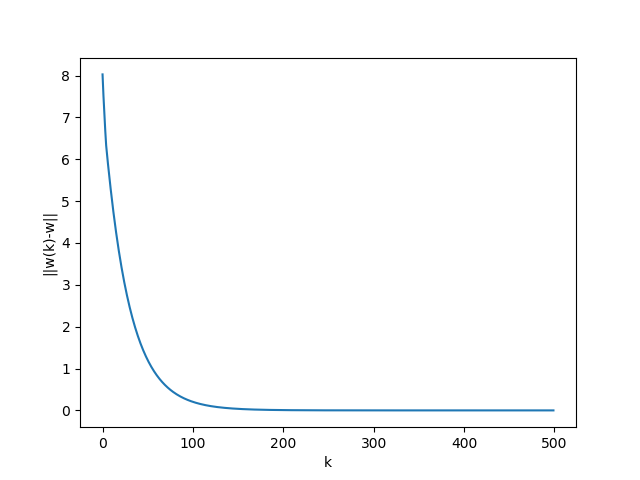
\includegraphics[width=\linewidth]{iterative.png}
		\caption{$\|w^{(k)}-\hat{w}\|$}
		\label{lsq}
	\end{figure}
	As you can see in the figure \ref{lsq}, the value of w is getting closer and closer to the optimal value of $\hat{w}$. After about 110 iterations, $w^{(k)}$ is converged with $\hat{w}$.
	
	
	%%%%%%%%%%%%%% TYPE YOUR SOLUTION ABOVE %%%%%%%%%%%%%%%%%%%%
	
	\subsection*{Problem 7. Logistic regression.}
	
	For this problem, you will use the IRIS dataset. Features are in the file IRISFeat.csv and labels in the file IRISlabel.csv. The dataset has 150 samples.
	A python script (name hw1-logistic.py) with all the steps need to be submitted. 
	
	\begin{enumerate}[label=\alph*)]
		\item (\textbf{12 Points})
		Your goal is to implement logistic regression. You can design or structure your code to fulfil the requirements but to get a full credit, the main script should output the required tables or plots with explicitly named x-y axis and the following function should be provided where X being features and y target.:
		\begin{itemize}
			\item [1.] Cross validation: Make sure you randomly shuffle the dataset and partition it into almost equal \textbf(k=5) folds. Save each of the 5 folds into dictionary  X\_shuffled and y\_shuffled.
			\newline
			X\_train, y\_train, X\_valid, y\_valid = get\_next\_train\_valid(X\_shuffled, y\_shuffled, itr) where itr is iteration number.
			\item[2.] model\_weights, model\_intercept = train(X\_train, y\_train)
			\item[3.] y\_predict\_class = predict(X\_valid, model\_weights, model\_intercept)
		\end{itemize}
		
		\textbf{USE GRADIENT DESCENT} to solve it. You should initialize the weights randomly to begin with.
		
		
		\item (\textbf{3 Points})
		At the beginning, briefly describe the approach in one paragraph along with any equations and methods used in your implementation. 
		
		
		\item (\textbf{5 Points})
		Report the plot of training and validation set error rates (number of misclassified samples/total number of samples) and the confusion matrix for validation set from 5-fold cross validation. 
		Explain your selection of learning rate and How does it affect the performance/training of your model? 
		
	\end{enumerate}
	
	\paragraph{Your answer.}
	\textbf{b) Following approach is used for training a logistic regression model}\\
	It has following functions:
	\begin{enumerate}
		\item \textbf{shuffle\_data\_in\_k\_folds:} It shuffles the features and labels data and divide it in k partitions.
		\item \textbf{get\_next\_train\_valid:} It return the training and validation sets for a given iteration.
		\item \textbf{train:} This method runs gradient descent algorithm for maximum of 1000 iterations or until the $\|dw\|_2^2 >= 0.001$ with learning rate of 0.1. model\_weights (W) and model\_intercept are updated using following equations\\
		\begin{enumerate}
			\item $dw = X^\intercal (y_i - \frac{1}{1+e^{-(w^\intercal X_i + b)}})$
			\item $db = y_i - \frac{1}{1+e^{-(w^\intercal X_i +b)}}$
			\item $w = w - \frac{1}{N}*learning\_rate * dw$
			\item $b = b - \frac{1}{N}*learning\_rate * db$
		\end{enumerate}
		\item \textbf{predict:} It uses following equation to predict the class given $X_i$\\
		$y = sign(\frac{1}{1+e^{-(w^\intercal X_i + b)}})$
	\end{enumerate}
	
	\paragraph{Your answer.}
	\textbf{c) Training and validation plots}
	
	\begin{enumerate}
		\item Plot of error rates for gradient descent:
			\begin{figure}[h!]
				\centering
				\begin{subfigure}[b]{0.4\linewidth}
					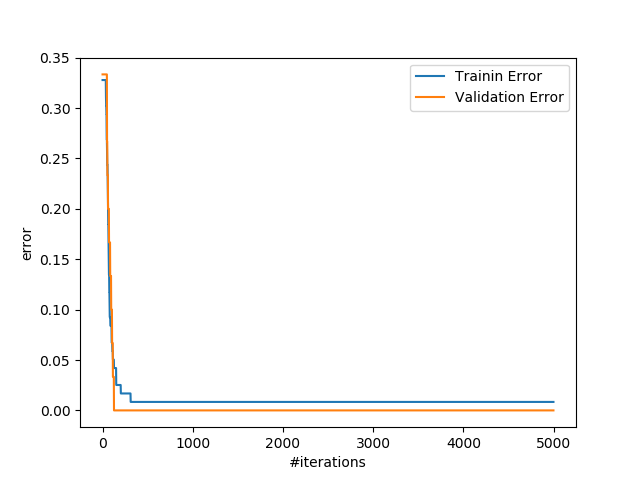
\includegraphics[width=\linewidth]{errorPlotFold1.png}
					\caption{Fold 1}
				\end{subfigure}
				\begin{subfigure}[b]{0.4\linewidth}
					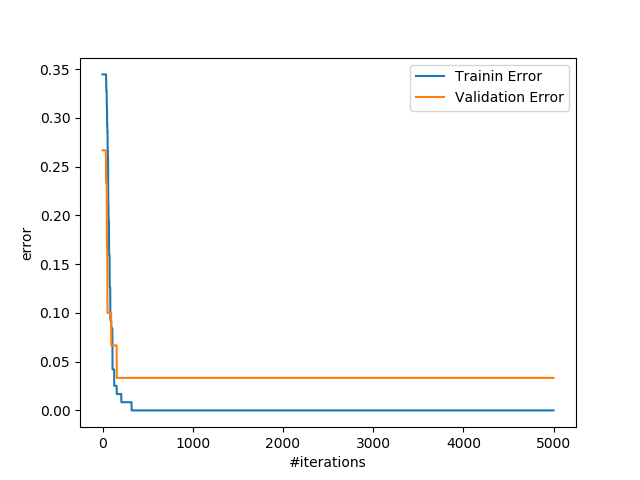
\includegraphics[width=\linewidth]{errorPlotFold2.png}
					\caption{Fold 2}
				\end{subfigure}
				\begin{subfigure}[b]{0.4\linewidth}
					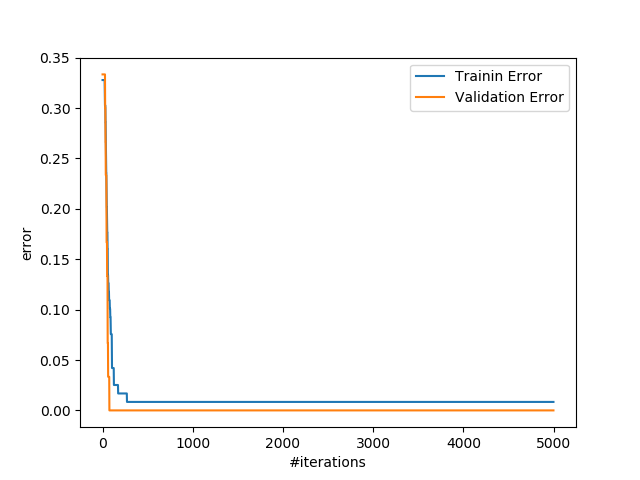
\includegraphics[width=\linewidth]{errorPlotFold3.png}
					\caption{Fold 3}
				\end{subfigure}
				\begin{subfigure}[b]{0.4\linewidth}
					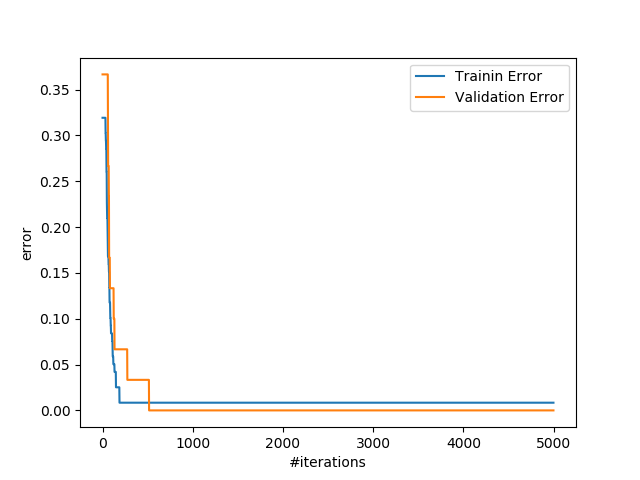
\includegraphics[width=\linewidth]{errorPlotFold4.png}
					\caption{Fold 4}
				\end{subfigure}
				\begin{subfigure}[b]{0.4\linewidth}
					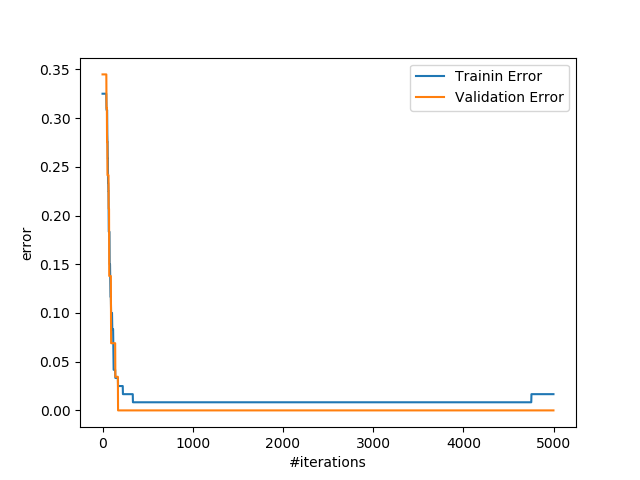
\includegraphics[width=\linewidth]{errorPlotFold5.png}
					\caption{Fold 5}
				\end{subfigure}
				\caption{Training and validation error rates}
			\end{figure}	
		\item Confusion matrices for 5 iterations:
			\begin{figure}[h!]
				\centering
				\begin{subfigure}[b]{0.4\linewidth}
					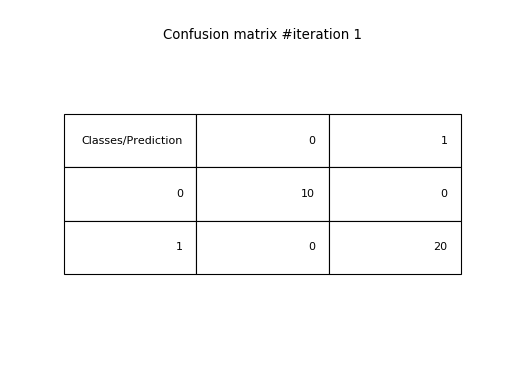
\includegraphics[width=\linewidth]{confusionMatrix1.png}
					\caption{Fold 1}
				\end{subfigure}
				\begin{subfigure}[b]{0.4\linewidth}
					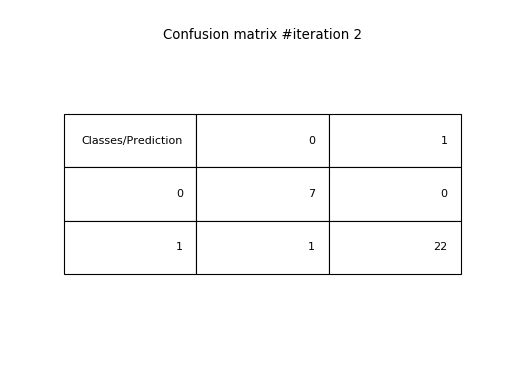
\includegraphics[width=\linewidth]{confusionMatrix2.png}
					\caption{Fold 2}
				\end{subfigure}
				\begin{subfigure}[b]{0.4\linewidth}
					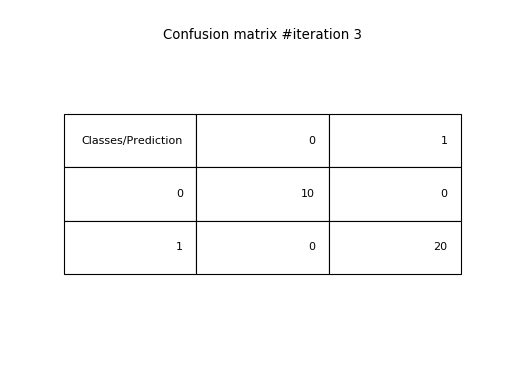
\includegraphics[width=\linewidth]{confusionMatrix3.png}
					\caption{Fold 3}
				\end{subfigure}
				\begin{subfigure}[b]{0.4\linewidth}
					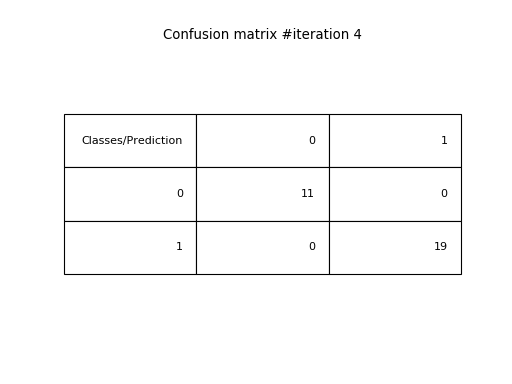
\includegraphics[width=\linewidth]{confusionMatrix4.png}
					\caption{Fold 4}
				\end{subfigure}
				\begin{subfigure}[b]{0.4\linewidth}
					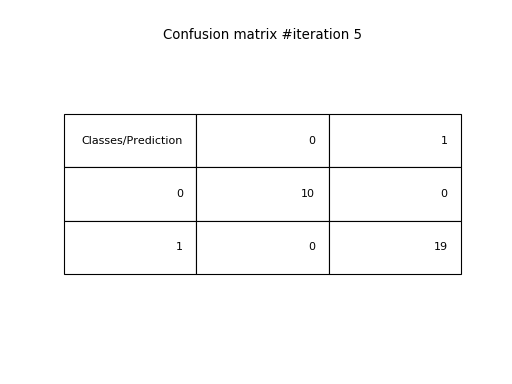
\includegraphics[width=\linewidth]{confusionMatrix5.png}
					\caption{Fold 5}
				\end{subfigure}
				\caption{Confusion matrix for validation set}
			\end{figure}	
	\end{enumerate}
	Number of iterations and learning rate were decided after running train method over a range of values. Tried learning rate in the range of (0.01 to 0.9), got best results at 0.1. Number of iterations were tested for the range(1000 to 5000). 5000 gave higher accuracy across all folds and also helped in converging to the optimal solution since our learning rate is relatively lower. Lower learning rate requires more iterations to converge, but higher learning rate even though takes less iterations, posses the risk of jumping over the optimum solution. Also low learning rate takes more time and high learning rate takes less time.
	
\end{document}